\section{Versuchsaufbau/-durchführung}
Der Versuchsaufbau, der sich in allen Teilen der Durchführung nur geringfügig unterscheidet, ist in Abbildung \ref{fig:aufbau} abgebildet.
Die Form der Generatorspannung $U\ua{G}$ wird dem jeweiligen Abschnitt der Messung angepasst.
\begin{figure}
  \centering
  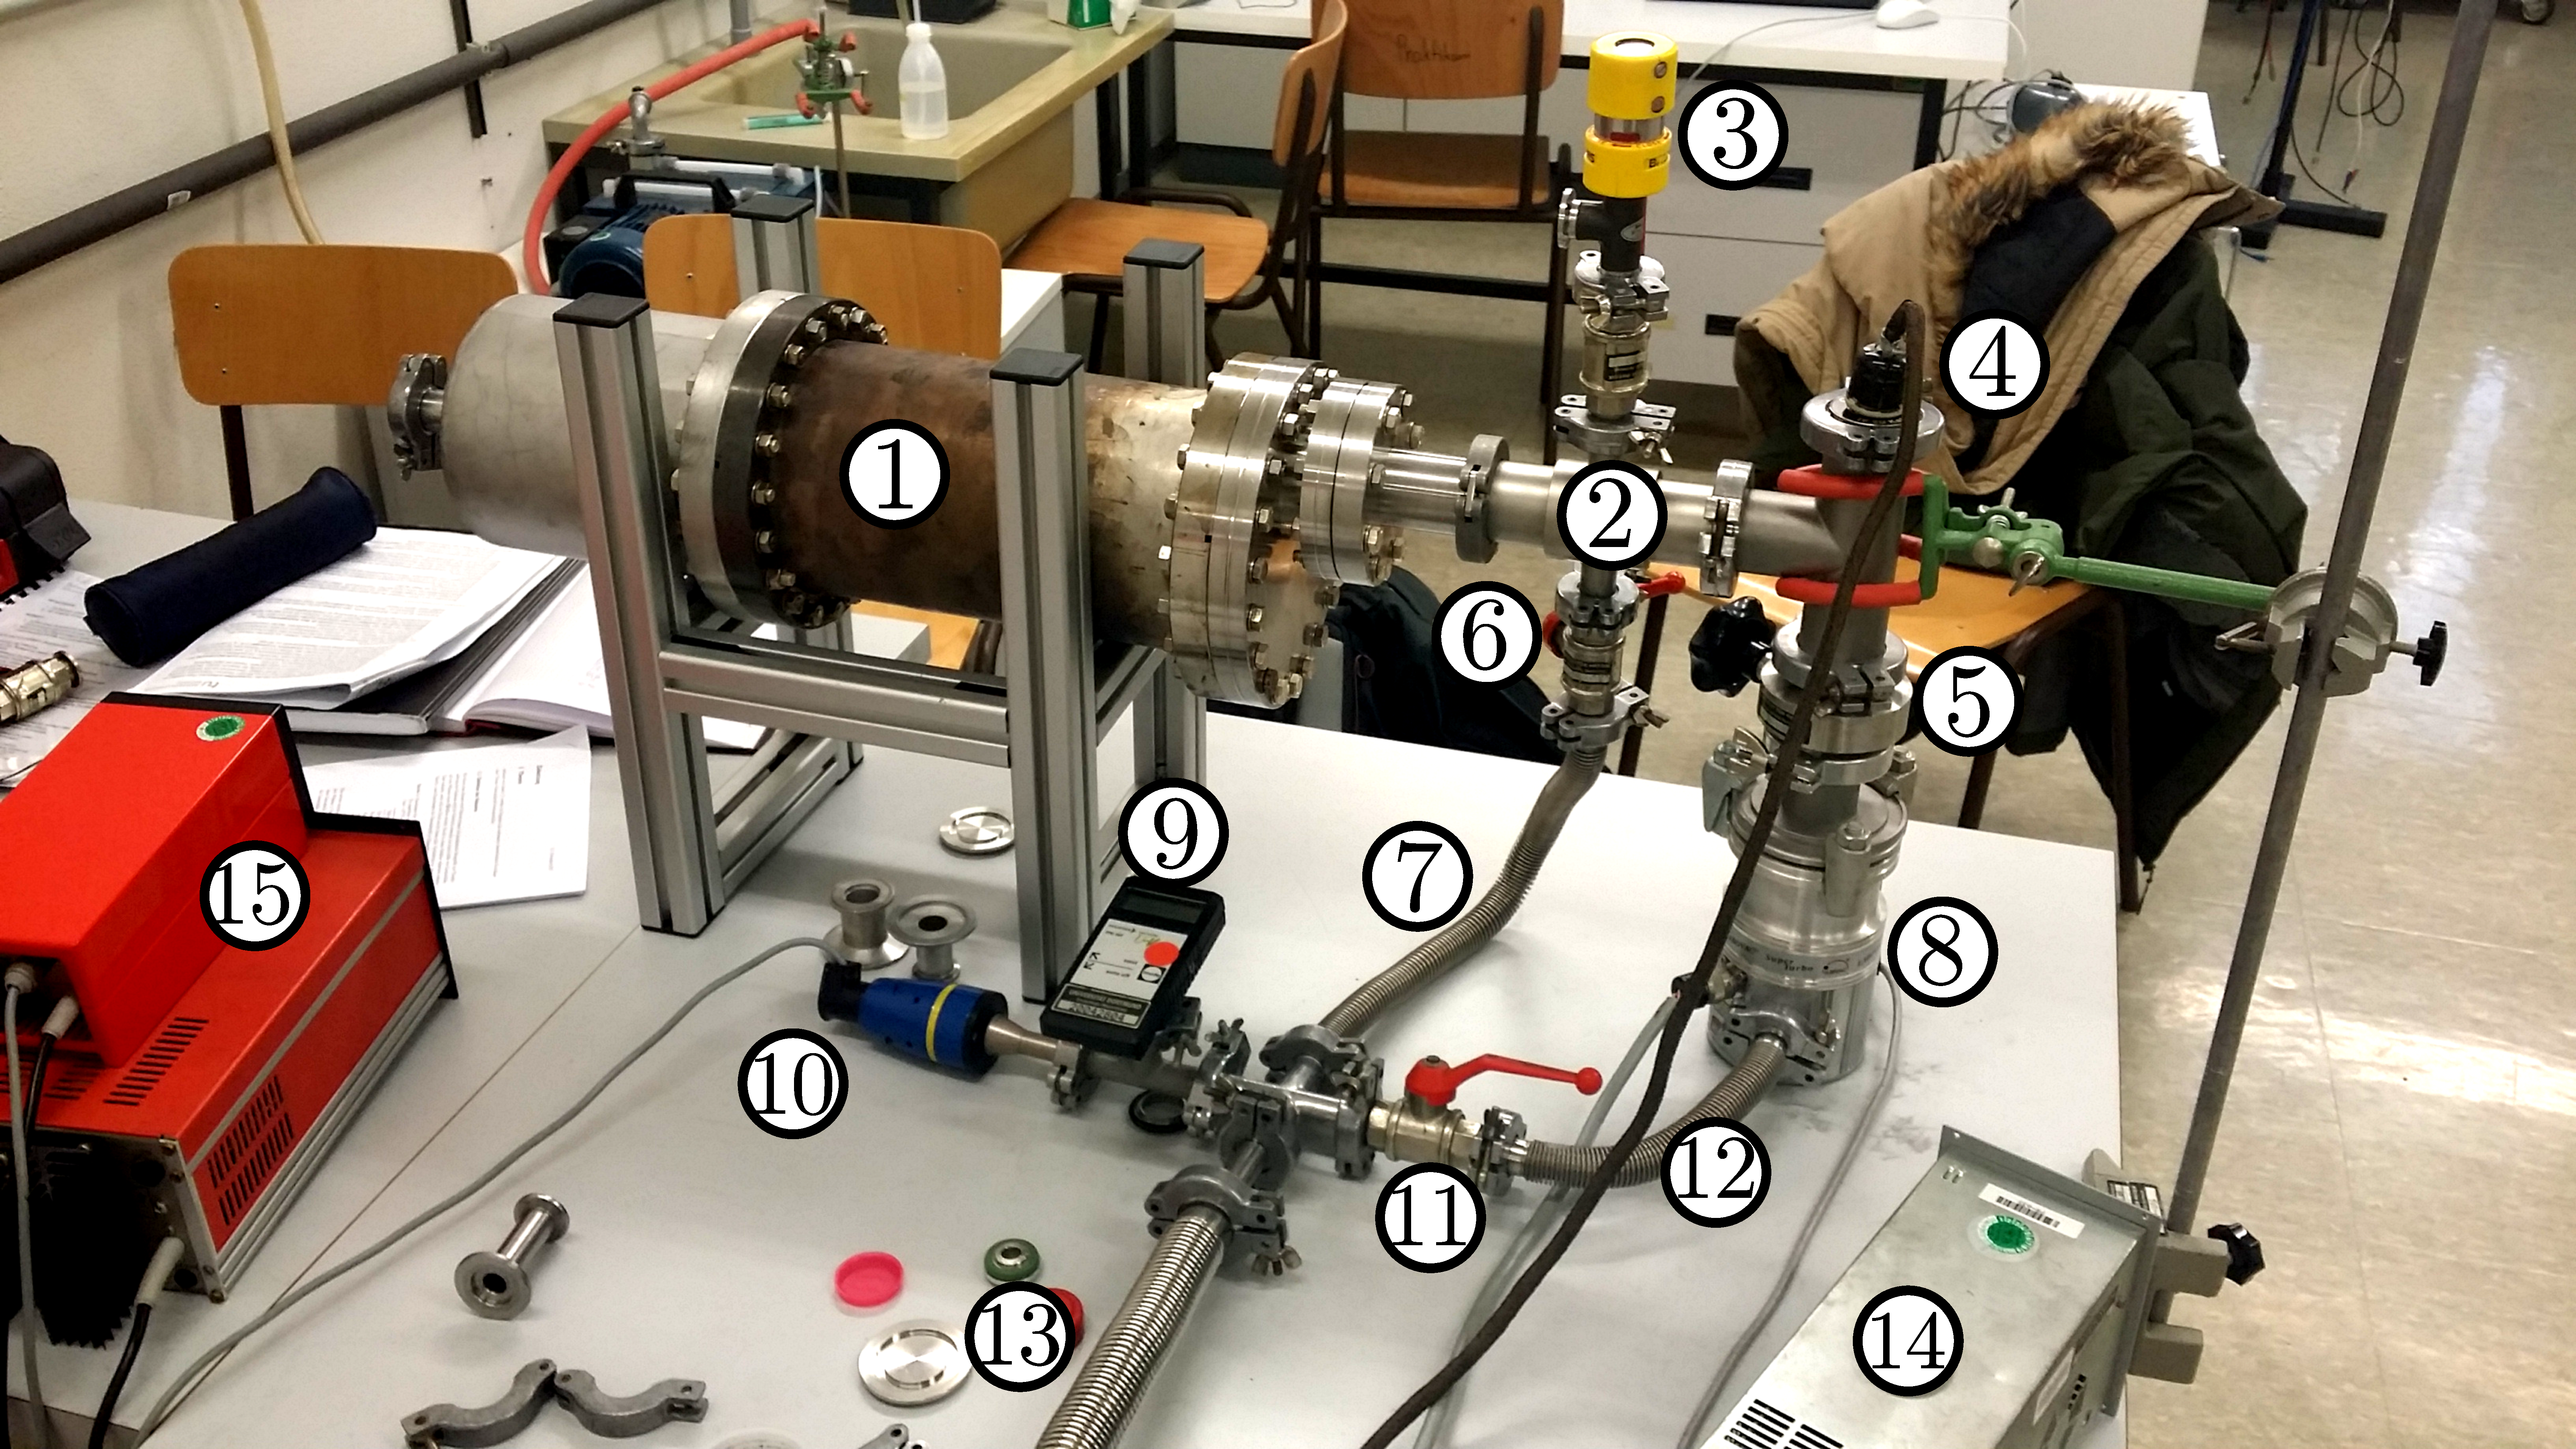
\includegraphics[width = 0.8\textwidth]{pics/aufbau.png}
  \caption{Aufbau zur Untersuchung des Relaxionsverhaltens eines RC-Gliedes \cite{anleitung207}}[bearbeitet].
  \label{fig:aufbau}
\end{figure}
\subsection{Bestimmung der Zeitkonstante}
Um die Zeitkonstante $RC$ zu bestimmen, wird am Generator G in Abbildung \ref{fig:aufbau} eine Rechteckspannung eingestellt.
Am Oszilloskop werden die Generatorspannung $U\ua{G}$ und die Entladekurve $U\ua{C}$ des Kondensators beobachtet und mittels eines Thermodrucks
dokumentiert.

\subsection{Untersuchung der Frequenzabhängigkeit von Phasenverschiebung und Amplitude}
Die
